\chapter{Bayes parameter extraction of complex model}
In the past three chapter, we have discussed the modeling details of the heavy flavor transport in the environment of the relativistic heavy-ion collisions.
And it is evident that the simulation requires a complex model with complex inputs.
To use such a model to acquire quantitative understanding about the properties of the quark-gluon plasma, we apply advanced statistical tools known as the Bayes analysis.
Let me first list out the problems one encounters in the model-to-data comparison in the field of heavy-ion collisions.

\paragraph{Complex dynamical model with high-dimensional inputs}
Taking the bulk model as an example, it includes an initial condition, a dynamical model for pre-equilibrium stage, the viscous hydrodynamics, particlization of the hydrodynamic energy momentum tensor and the hadronic decays and rescatterings.
Each of the module takes both physical parameters and modeling parameters.
Eventually, one can have more than 10 parameters.
To generate one event with a model itself is already computationally intensive, while to be able to compare to experimental measurements that average over centrality with a good control of statistical uncertainty, $O(10^4)$ minimum-biased events needed to be generated.
As a result, a na\"ive linear grid sweep over the 10-dimensional parameter space is certainty not feasible.
To solve this problem of high-dimensional input complex models requires advanced parameter set design method and reliable interpolation schemes.

\paragraph{Model uncertainty and correlation among parameters}
We are mostly interested in those ``physical parameters / quantities'', for example, the transport coefficients $\eta/s(T)$ and $\zeta/s(T)$ of the medium.
Other parameters, such the switching time between the pre-equilibrium free-streaming dynamics and the hydrodynamics, and the temperature at which one particlize a hydrodynamic field description into a hadronic ensemble are less interested in the physical sense.
The appearance of these matching parameters are simply due to we do not have a single ``global model'' that works reasonably well under all circumstances.
However, one should not think less of these model parameters, because the quantify a significant fraction of the modeling uncertainty.
The model uncertainty can affect the interpretation of the experimental data, and any quantitative statement we draw about those physical quantities from a model-to-data comparison.
For example, the  bulk particles anisotropic flows, though proved to be very sensitive to the shear viscosity, are also sensitive to the initial eccentricity of the initial conditions.
Therefore, the exacted $\eta/s$ becomes correlated with the choice of initial condition models and its parameters.
The model uncertainty is hard problem, and one can either try to reduce it by improving the model or quantify it when compared to data to prevent an over-interpretation.

\paragraph{A high-dimensional model output / observables}
The inclusion of more observables also helps to break the model degeneracy and parameter correlation.
But it can be tricky to quantify the quality of agreement between model and data with a collection of observables (a high dimensional output).


The Bayesian analysis framework is introduced to the field by the earily works of and the PhD thesis of Jonah Bernhard [] who has successfully applied the tool to the extraction of the initial condition topology and temperature dependent QGP transport coefficient.
This chapter provides a concise description of the Bayesian analysis and for full details please refer to the thesis of Jonah Bernhard [].

We abstract the general task of a model-to-data comparison into the following form,
\begin{itemize}
\item A complex model $M$, with input parameters organized as a vector $p$ of dimensional $m$.
\item There are certain prior belief on the reasonable range of each parameters, known as the prior probability distribution $\mathrm{Prior}$.
\item The experimental data are organized as an observation vector $y_{\exp}$ of dimensional $n$
\item Goal: to infer the probability distribution of $p$, given the model $M$, the measurements $y_{\exp}$, and the prior belief $\mathrm{Prior}$. The resultant distribution is called the posterior probability distribution $\mathrm{Posterior}$.
\end{itemize}

\section{The design of parameters}
The first step is an understanding of the behavior of the model $M$.
This is done by sampling the high-dimensional input parameter space with a finite number of design parameter set.
Mathematically, this $N$ set of parameter vectors of length $n$ forms a so-called design matrix $\mathbf{D}$,
\begin{eqnarray}
\mathbf{D}_{N\times n} = 
\begin{bmatrix}
p_{11} & p_{12} & \cdots & p_{1n}\\
p_{21} & p_{22} & \cdots & p_{2n}\\
\vdots & \vdots & \ddots & \vdots \\
p_{N1} & p_{N2} & \cdots & p_{Nn}
\end{bmatrix}
\end{eqnarray}
where the first index is the label of different parameter set, and the second index labels different parameters.
We want an efficient sampling of the design points, so that the number of $N$ is manageable while still provide a representative coverage of the entire parameter space.
We used Latin-Hyper-Cube sampling method, it generate a random design but subject to the following constraint:
\begin{itemize}
\item The marginalized distribution on any parameters is a uniform distribution. This is different from a grid design, where the marginalized distribution are spiky delta function on the grid points.
\item The minimum distanced between any two point in the parameter space is maximized. This is different from a complete random design, where the points may from tight cluster or sparse regions.
\end{itemize}
Usually, for a well behaved model, the number of design points needed for a good interpolation increases linearly with the number of parameters, in contrast to the exponential increase with number of parameters for a grid design.

Once the design is made, the time consuming part is then to perform the full model calculation on each points and organize all the computed observables into an observation matrix,
\begin{eqnarray}
\mathbf{Y}_{N\times m} = 
\begin{bmatrix}
y_{11} & y_{12} & \cdots & y_{1m}\\
y_{21} & y_{22} & \cdots & y_{2m}\\
\vdots & \vdots & \ddots & \vdots \\
y_{N1} & y_{N2} & \cdots & y_{Nm}
\end{bmatrix}
\end{eqnarray}
where the first index is the label of different parameter set, and the second index labels different observables.
The design matrix $\mathbf{D}$ and the observations matrix $Y$ forms the training data to build a general interpolator for the mapping from the parameter space to the observable space $M: \vec{p} \rightarrow \vec{y}(\vec{p})$.

\section{Data reduction}
The model $M$ is an $n$-dimesional vector to an $m$-dimensional vector mapping. 
One can certainly construct an independent array of $m$ scalar mappings, and interpolate each of them using the training data.
However, this na\"ive construction does not make use of the intrinsic correlations / structures that is already presented in the training data, and can be very inefficient for practice usage.
For example, consider the observations contain two values of $R_{AA}$ and $v_2$ for $D$-meson, and usually the larger the $R_{AA}$ is, the smaller the $v_2$, and thus an anti-correlation is expected.
If one build interpolators for $R_{AA}$ and $v_2$ independently, their uncertainty is also going to be independent, and the intrinsic correlation is overlooked.
However, if one choose to interpolates the linearly combinations $a R_{AA} \pm b v_2$, then a wise choice of $a, b$ can largely reduces the correlation between these two ``new" observables.

The principal component analysis (PCA) is the systematic way to implement this idea.
The original vectors of observables are transformed into the principal-component (PC) space, with each PC a specific linear combination of the original observables, so that the covariances between the newly defined observables (the PCs) vanish.
Mathematically, this is the same as finding the singular value decomposition (SVD) of $\mathbf{\tilde{Y}}$. 
$\mathbf{\tilde{Y}}$ is the standardized observation matrix $\mathbf{Y}$,
\begin{eqnarray}
\tilde{y}_{ij} = \frac{y_{ij} - \mu_j}{\sigma_j}
\end{eqnarray}
with $\mu_j$ and $\sigma_j$ the mean and the standard deviation of column $j$.
Then the SVD proceeds as,
\begin{eqnarray}
\tilde{\mathbf{Y}} = \mathbf{U} \mathbf{\Sigma} \mathbf{V}
\end{eqnarray}
And the principal components are defined as the components after the $V$ transformation.
\begin{eqnarray}
z = \mathbf{V}y
\end{eqnarray}
It is evident that the covariance matrix of the $z$ observables are diagonalized,
\begin{eqnarray}
\mathrm{Var}(z_i, z_j) = \frac{1}{N}V_{ii'}\tilde{Y}_{ki'}V_{jj'}\tilde{Y}_{kj'} = \frac{1}{N}V\tilde{Y}^T\tilde{Y}V^T = \frac{1}{N}\mathbf{\Sigma}
\end{eqnarray}
so that the PCs are orthogonalized.
One more benefits is that, suppose the variance in $\Sigma$ has been ordered from maximum to minimum.
For data with pronounced structures, often the first few principal components take account the majority of the data variance.
And for practical usage, a truncation of the number of PCs already gives a good representation of the original data, and this greatly reduces the computations for large number of observables.
In the end, one can always go back from the PC space to the original physical space by $y = V^{-1} z$.

\section{Model emulator}
With limited information on a finite number of design points contained in the matrices $D$ and $M$, the original mapping is approximated by a model emulator (a surrogate model) using the Gaussian process.
The Gaussian process provide a non-parametric interpolation for scalar function and also works for high dimensional input.
The 




\section{Model calibration using Bayesian analysis}\label{section:calibration}
Finally, we couple our transport model to a state-of-the-art 2+1D event-by-event viscous hydrodynamical medium evolution and extract the model parameters from a Bayesian model-to-data comparison.
The medium evolution model consists of multiple stages,
\begin{itemize}
\item[1.] The \trento\ model generates event-by-event initial conditions at time $\tau = 0^+$ {Moreland:2014oya}. 
\item[2.] A collision-less Boltzmann equation (free streaming) models the pre-equilibrium stage prior to the start of the hydrodynamic evolution at $\tau_{fs}$ {Liu:2015nwa}.
\item[3.] 2+1D event-by-event relativistic viscous hydrodynamics evolves the QGP with an up-to-date lattice equation of state (EoS) {Shen:2014vra, Bazavov:2014pvz}.
\item[4.] Finally, hadrons sampled from hydrodynamic energy momentum tensors rescatter and decay in the hadronic phase utilizing the Ultra-Relativistic Quantum Molecular Dynamics (UrQMD) model {Bass:1998ca, Bleicher:1999xi}.
\end{itemize}
The parameters of this particular bulk medium evolution have already been calibrated to reproduce a vast array of bulk observables at LHC energies {Bernhard:2018hnz}, providing a description of the bulk evolution of the QGP with unprecedented precision.
On the heavy quark transport side, we initialize heavy quark ensembles with momenta sampled from a FONLL calculation using two different sets of nuclear parton distribution functions (PDFs) {Cacciari:1998it,Kovarik:2015cma,Eskola:2016oht}. 
The nuclear PDFs comes with a large uncertainty in the shadowing region which is relevant at the LHC energies.
It is hard to systematically include this uncertainty in our study; instead, we choose to use the center values of two different sets of nuclear PDFs, namely the {\tt EPPS} set and the {\tt nCTEQ16np} set and perform calibrations using both to demonstrate the sensitivity of the parameter extraction on the nuclear PDF uncertainty.
The position of the hard production vertices at $\tau = 0^+$ are sampled from the \trento\ binary collision density to correlate with hot-spots of  underlying event. 
During the pre-equilibrium stage, the heavy quarks should already start to interact with medium.
However, the system at this stage is still far off both kinetic and chemical equilibrium.
To get a handle on the effect of pre-equilibrium energy loss, we choose to define the medium flow velocities and energy density from the pre-equilibrium energy-momentum tensor by Landau matching and convert the energy density to an effective temperature using a three-flavor conformal QCD EoS. 
Heavy quarks are allowed to loose energy from a tunable energy-loss starting time $0.1< \tau_0 < 1.0 \textrm{ fm/$c$} $. 
With a small $\tau_0$, this correspond to a fast generation of color degrees of freedom in the medium that can collide with heavy quarks at very early times, and with a large $\tau_0$ the pre-equilibrium effects are gradually turned off.
This is of course a rather crude setup and in the future we plan on utilizing more sophisticated models based on kinetic theory to treat pre-equilibrium stage energy loss {Srivastava:2017bcm}.
During the hydrodynamic expansion, the evolution of the flow velocities and temperature are provided by the 2+1D viscous hydrodynamics with boost-invariance in the beam direction.
The heavy quarks subsequently hadronize using a sudden-approximation at $T = 0.154$ GeV via fragmentation and recombination mechanisms {Cao:2013ita}. 
B mesons cease to interact at this point in our model, but D mesons are included in the UrQMD afterburner with $\pi$-D and $\rho$-D cross-sections {Lin:2000jp}.

The parameters of our model in the heavy-flavor sector are:
\begin{itemize}
\item[1.] $\tau_0$ the time at which heavy quark energy loss starts, varying between $0.1$ fm/$c$ to $1.0$ fm/$c$,
\item[2.] $\mu$, the medium energy scale ($\mu\pi T$) that appears in the running coupling constant of the scattering component, varying from $1/3$ to $4$,
\item[3.] $\kappa_D$, the strength of momentum diffusion at $ET = 1 \textrm{GeV}^2$, ranging from $0$ to $8$, and
\item[4.] $x_D$, the fraction of the momentum diffusion that is energy independent, ranging from $0$ to $1$.
\end{itemize}
In addition to these continuous parameters, the choice of different nuclear parton distribution functions acts as a discrete variable.

We now briefly introduce the Bayesian techniques and key terminologies to be used later. These techniques have been described in great detail in a series of publications regarding their application to the extraction of bulk QGP properties and initial conditions of heavy-ion collisions {Bernhard:2015hxa,Bernhard:2016tnd} as well as in the heavy quark sector to the extraction of the heavy quark diffusion coefficient within the framework of an improved Langevin transport model {Xu:2017obm}.
The application of these techniques to relativistic heavy-ion collisions in general has been part of the 
thesis work by J. Bernhard {Bernhard:2018hnz}.

Given a model whose prediction ${\bf y}$ depends on a vector of input parameters ${\bf p}$ and  experimental data ${\bf y}_\textrm{exp}$, 
the probability distribution of the {\it true} model parameters ${\bf p^*}$ is given by Bayes' theorem, 
\begin{eqnarray}\label{eq:Bayes}
\textrm{Posterior}({\bf p^*}|{\bf y}_\textrm{exp}, M) &\propto& \textrm{Likelihood}({\bf y}_\textrm{exp}|{\bf p^*}, M) \nonumber \\ &\times& \textrm{Prior}({\bf p^*}).
\end{eqnarray}
The posterior probability distribution of the ${\bf p^*}$ given a certain model $M$ and data, equals the probability $L$ of observing the data given the model and parameters ${\bf p^*}$, called likelihood function, times a prior belief on the distribution of ${\bf p^*}$.
The likelihood function is often defined in a Gaussian form in terms of the difference between model calculation and experimental data and a covariance matrix $\Sigma$ that encodes experimental and theoretical uncertainties,
\begin{eqnarray}\label{eq:likelihood}
\ln(L) &=& -\frac{1}{2}({\bf y}-{\bf y}_{\textrm{exp}})^T\Sigma^{-1} ({\bf y}-{\bf y}_{\textrm{exp}})\nonumber\\ 
		&-&\frac{d}{2}\ln(2\pi)-\frac{1}{2}\ln|\Sigma|.
\end{eqnarray}
The construction of $\Sigma$ is described in Appendix \ref{appendix:sigma}.
Once we have the ability to evaluate model output given arbitrary parameters within a reasonable range, the information on the parameters constrained by data follows from Equations (\ref{eq:Bayes}) and (\ref{eq:likelihood}).
This high-dimensional posterior probability distribution function can be sampled using a Markov-chain Monte Carlo (MCMC) procedure.
The main challenge for applying this method directly to event-by-event heavy-ion collision models resides in the computational effort required for the model calculations.  $\mathcal{O}(10^4)$ minimum-biased events are needed to get statistical uncertainties of the calculation under control.
Since it is impractical to evaluate the model  at arbitrary points in parameter space during the MCMC sampling, alternative methods for rapid model evaluations have to be found.
The solution is to use an advanced sampling technique by only evaluating the full model at $\mathcal{O}(100)$ design parameter sets (design points) and subsequently interpolating the model to generate output at arbitrary points in parameter space using  Gaussian process emulators that have been trained on the full model calculation at the design points {Rasmussen:2006gp}.
\begin{center}
\begin{table}[h]
\caption{ALICE dataset}\label{table:ALICE-obs} 
\begin{tabularx}{\columnwidth}{XXX}
\hline 
 Observables & Centrality & Reference\\ 
\hline 
$D$-meson $v_2$ & 30-50\% & {Acharya:2017qps}\\ 
\hline 
Event-engineered $D$-meson $v_2$ & 30-50\% & {Grosa:2017zcz}\\ 
\hline 
$D$-meson $R_{AA}$ & 0-10, 30-50, 50-80\% & {Acharya:2018hre}\\
\hline 
\end{tabularx}
\end{table}
\begin{table}[h]
\caption{CMS dataset}\label{table:CMS-obs} 
\begin{tabularx}{\columnwidth}{XXX}
\hline 
Observables & Centrality & Reference\\ 
\hline 
D${}^0$-meson $v_2$ & 0-10, 10-30, 30-50\% & {Sirunyan:2017plt}\\ 
\hline 
D${}^0$-meson $R_{AA}$ & 0-10\%, 0-100\% & {Sirunyan:2017xss}\\ 
\hline 
B${}^{\pm}$-meson $R_{AA}$ & 0-100\% & {Sirunyan:2017oug}\\ 
\hline 
\end{tabularx}
\end{table}
\end{center}

In this work, we sampled 80 design points in a four dimensional parameter space $(\tau_0, \mu, \kappa_D, x_D)$.
For each parameter set, we run 4000 minimum bias events.
Each event propagates an ensemble of $4\times 10^4$ charm quarks and $10^4$ bottom quarks.
The centrality is defined by the mid-rapidity charged particle multiplicity and the same kinematic cuts as are used by the experiments are applied to the calculation of heavy-flavor observables.
All observables are measured at 5.02 TeV in Pb+Pb, as listed in Table \ref{table:ALICE-obs} and \ref{table:CMS-obs}. Most of the data we utilize are for $D$-mesons: the
 $p_T$ dependent $D$-meson nuclear modification factor $R_{AA}$ and $p_T$ dependent second-order azimuthal anisotropy $v_2$ at various centralities {Sirunyan:2017plt, Sirunyan:2017xss, Acharya:2017qps,Grosa:2017zcz}.
We also compare to the event-shape-engineered $D$-meson $v_2$ measured by the  ALICE collaboration {Grosa:2017zcz}.
The idea of the event-shape engineering is to subdivide events at a certain centrality according to the magnitude of the charged particle $q$-vector, in this case,
\begin{eqnarray}
|q_2|^2 = \frac{\left(\sum_{i=1}^{M} \cos(2\phi) \right)^2+ \left(\sum_{i=1}^{M} \sin(2\phi) \right)^2}{M} \, .
\end{eqnarray}
The $D$-meson $v_2$ is measured for those events with $20\%$ highest $q_2$ and events with $60\%$ lowest $q_2$.
It is found that $D$-meson flow is strongly correlated with this measurement of bulk collectivity.
This event-shape-engineering procedure necessitates a full event-by-event study and may be sensitive to the interplay between heavy quark energy loss and initial condition fluctuations, so we include this observable into the set of observables on which we calibrate the model.
Finally in order to require the calibrated model to predict the desired mass-dependence, we include recent CMS measurements of $B^{\pm}$-meson $R_{AA}$, although the data have a large uncertainty which suppresses its importance in the likelihood function.
\begin{figure*}
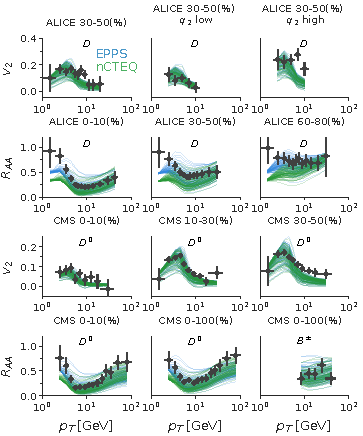
\includegraphics[width=.49\textwidth]{observables_design.pdf}
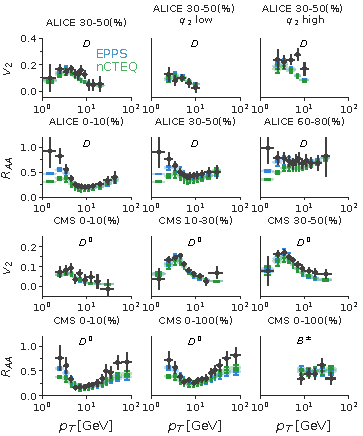
\includegraphics[width=.49\textwidth]{observables_posterior.pdf}
\caption{Left: the prior, i.e. the full range of calculations in parameter space. Right: the posterior, i.e. observables sampled from model emulators after calibration. In both figures, blue (green) lines are calculations with {\tt EPPS} ({\tt nCTEQ15np}) nuclear PDF.}\label{plots:deisgn_posterior_obs}
\end{figure*}

On the left of Figure \ref{plots:deisgn_posterior_obs}, we show the prior, i.e. the full range of our calculations in parameter space for each of the listed observables. 
We use different colors to distinguish calculations using {\tt EPPS} (blue) and
{\tt nCTEQnp} (green) nuclear PDF.
The calculated values of $R_{AA}$ at high transverse momenta and $v_2$ at low transverse momenta have a large spread, sufficiently wide to cover the experimental data.
We notice that the model always underestimates very low-$p_T$ $R_{AA}$ points and 30-50\% high-$p_T$ $v_2$ from CMS.
This could be a limitation of our model, such as the need of a more sophisticated implementation of the LPM effect or the need for a more accurate calculation of initial low-$p_T$ charm quark production in both $p$-$p$ and $A$-$A$ collisions. 
Plots on the right of Figure \ref{plots:deisgn_posterior_obs} show the posterior distribution of the observables from model emulators, i.e. interpolated model predictions after calibration.
The calibrated model displays a very good overall agreement with all the observables except for the cases pointed out above.
The use of different nuclear PDFs has a  negligible effect on azimuthal anisotropy observables, but does affect the $R_{AA}$ at small and large $p_T$.
Calculations with the {\tt EPPS} nuclear PDF work very well in describing $R_{AA}$ below $p_T = 50$ GeV, while calculations with the {\tt nCTEQnp} do slightly better for CMS $R_{AA}$ data with $p_T>50$ GeV.
The calculated event-engineered flow strongly correlates with the charged particle $|q_2|$ and describes the lowest 60\% $q_2$ bin very well.
For the highest 20\% $q_2$ bin, the model posterior is consistent with measurements below $5$ GeV and underestimates the data at higher $p_T$ bins.

\begin{figure}
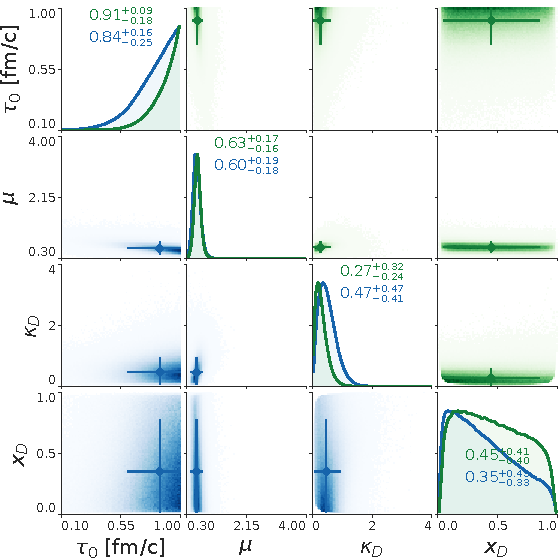
\includegraphics[width=.5\textwidth]{posterior.pdf}
\caption{Marginalized postrior probability distribution of model parameters. Diagonal plots show the marginalization on a single parameter. Off diagonal plots show the pair correlation between parameters. Blue (Geen) lines and lower (upper) off diagonal plots correspond to the extraction using EPPS (nCTEQ15np) nuclear PDF.}\label{plots:posterior}
\end{figure}
\begin{figure}
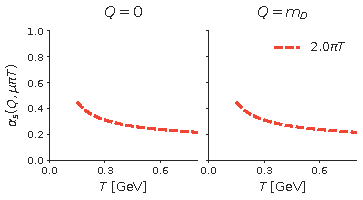
\includegraphics[width=.5\textwidth]{alpha_s_at_T.pdf}
\caption{Coupling constant with three values of the medium scale parameter $\mu$ taken  from the high likelihood region of the posterior. Left: $\alpha_s$ evaluated at a process scale $Q=0$. Right: $\alpha_s$ evaluated at a process scale $Q=m_D$.}\label{plots:alphas}
\end{figure}

The posterior probability distribution of all parameters is marginalized to single parameter distributions (diagonal) and two-parameter joint distributions (off-diagonal) in Figure \ref{plots:posterior}.
The lower off-diagonal plots and blue lines in the diagonal plots correspond to the calibration using the {\tt EPPS} nuclear PDF, and the upper off-diagonal plots and green lines in the diagonal plots use the {\tt nCTEQ15np} nuclear PDF.
Despite the difference in $R_{AA}$ when different nuclear PDFs are used, the extracted probability densities of parameters are similar.
To describe LHC data, the model prefers a late onset of medium induced energy loss and a medium energy scale roughly around $0.6\pi T$, which implies the largest coupling constant at a given temperature is $\alpha_s \sim \alpha_s(1.8T)$.
A small but finite amount of momentum diffusion at $ET=1\textrm{ GeV}^2$ is preferred for the diffusion component.
The smallness of this number is expected since most of the interaction is already taken account by the pQCD scattering component with a relatively large coupling constant (i.e. a small medium scale).
We find this study to be not sensitive to the energy / temperature dependence of the diffusion component beyond the regular $T^3$ scaling of the momentum diffusion constant.   

The preferred medium scale parameter $\mu \sim 0.6$ is not large which could result in a large $\alpha_s$.
Therefore, we check the range of typical $\alpha_s$ values in the model in order to evaluate the use of perturbative matrix-elements.
Figure \ref{plots:alphas} shows the coupling constant evaluated at two process scales $Q=0$ and $Q=m_D$.
In the case of $Q=0$ (left), the energy scale is cut off by $\mu\pi T$ and this plot show the maximum of model coupling constant at a given temperature.
Setting $Q=m_D$ (right) as a proxy for the typical momentum transfer in the $t-$channel scattering, the coupling constant rises slower as temperature drops.
It is found that in order to describe experimental data, the preferred coupling constant is fairly large, suggesting next-to-leading (NLO) order corrections to the present scattering picture should be prominent. 
Because these large $\alpha_s$ values are encountered in small-momentum-transfer scatterings ($0< Q < m_D$), we will absorb these small-momentum-transfer elastic and inelastic pQCD processes into a radiation-improved Langevin equation in future studies. 
This way, one not only avoids the explicit use of large $\alpha_s$ in pQCD matrix-elements, but also interpolates between the pQCD based scattering model, the radiation-improved Langevin model and pure non-perturbation drag and diffusion model with one or two control parameters, allowing for more systematic model-uncertainty study.

Next, we investigate the transport coefficients extracted from the calibrated model.
To define the transport coefficient of a heavy quark,
we combine the contribution from both elastic scatterings and the diffusion component,
\begin{eqnarray}\label{eq:qhat}
\frac{\hat{q}}{T^3} &=& \frac{1}{T^3}\frac{d}{dt}\left\langle p_\perp^2 \right\rangle\\
\nonumber
 &=&  \kappa_D\left(x_D + (1-x_D)\frac{\textrm{GeV}^2}{ET}\right) + \frac{\hat{q}_{\textrm{el}}}{T^3}.
\end{eqnarray}
Where $\hat{q}_{\textrm{el}}$ is obtained by integrating the rate equation with inserting the transverse momentum transfer square.
We shall discuss the inclusion of inelastic process into the calculation of $\hat{q}$ in section \ref{section:conclusion}.
Performing this calculation for many random parameter set samples drawn from the posterior distribution using either nuclear PDF, we determine the posterior distribution of the functional $\hat{q}(E, T)$ constrained by data.
On the left of Figure \ref{plots:posterior_qhat}, we showed the 95\% credible region of $\hat{q}$ as function of temperature, fixing the heavy quark momentum at $10$ GeV.
The right panel of the figure shows $\hat{q}$ as function of momentum at $T=0.35$ GeV.
Our formula includes a mass dependence -- therefore  the charm quark $\hat{q}$ (region enclosed by thick red lines and slashes) is slightly different from the bottom quark $\hat{q}$ (region enclosed by thick blue lines).
The present result is consistent with previous work by Xu et al (shaded region) {Xu:2017obm}, who used an improved Langevin model to extract the charm quark transport properties at the LHC,  but hits the lower half of the 95\% credible region of the previous extraction.
\begin{figure}
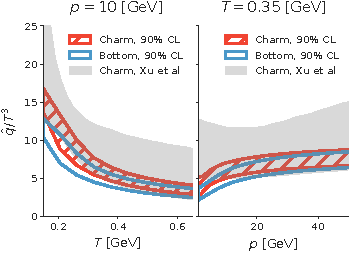
\includegraphics[width=\columnwidth]{qhat_p_T.pdf}
\caption{Posterior range of the heavy quark transverse momentum broadening parameter $\hat{q}$ from Equation \ref{eq:qhat}. The results include the uncertainty from using different nuclear PDFs. Blue boxed region is for bottom quarks and red slashed region for charm quarks. The shaded region indicates a previous extraction {Xu:2017obm}.}\label{plots:posterior_qhat}
\end{figure}
Alternatively, one can present our results in terms of the heavy quark spatial diffusion constant $D_s$ often defined in the limit of $p\ll M$.
It is related to the momentum diffusion parameter by
\begin{eqnarray}
2\pi T D_s = \frac{8\pi T^3}{\hat{q}(p\rightarrow 0, T)} \, .
\end{eqnarray}
In figure \ref{plots:posterior_Ds}, we plot the 95\% credible region of both the charm (region enclosed by red thick lines and slashes) and bottom (region enclosed by blue tick lines) quark spatial diffusion constant as function of $T/T_c$.
The results of this work is systematically higher than the extraction from the former work (shaded region).
There have also been attempts made to calculate the spatial diffusion constant of heavy quarks using lattice QCD: three calculations are available, two are calculated in the static heavy quark limit (blue and black symbols with higher values) {Banerjee:2011ra, Banerjee:2011ra}, one of which performs continuum extrapolation (black square) {Francis:2015daa}; the other result uses a realistic charm quark mass (red triangle symbols with lower values) {Ding:2012sp}.
Our posterior of $D_s$ including the diffusion contribution but with only elastic scattering agrees with the lattice evaluation in the static heavy quark limit.
The effect of including the inelastic scattering in $D_s$ will be discussed in the last section.



